%% Nothing to modify here.
%% make sure to include this before anything else

\documentclass[10pt]{beamer}
\usetheme{Szeged}

% packages
\usepackage{color}
\usepackage{listings}

% color definitions
\definecolor{mygreen}{rgb}{0,0.6,0}
\definecolor{mygray}{rgb}{0.5,0.5,0.5}
\definecolor{mymauve}{rgb}{0.58,0,0.82}

% re-format the title frame page
\makeatletter
\def\supertitle#1{\gdef\@supertitle{#1}}%
\setbeamertemplate{title page}
{
  \vbox{}
  \vfill
  \begin{centering}
  \begin{beamercolorbox}[sep=8pt,center]{title}
      \usebeamerfont{supertitle}\@supertitle
   \end{beamercolorbox}
    \begin{beamercolorbox}[sep=8pt,center]{title}
      \usebeamerfont{title}\inserttitle\par%
      \ifx\insertsubtitle\@empty%
      \else%
        \vskip0.25em%
        {\usebeamerfont{subtitle}\usebeamercolor[fg]{subtitle}\insertsubtitle\par}%
      \fi%     
    \end{beamercolorbox}%
    \vskip1em\par
    \begin{beamercolorbox}[sep=8pt,center]{author}
      \usebeamerfont{author}\insertauthor
    \end{beamercolorbox}
    \begin{beamercolorbox}[sep=8pt,center]{institute}
      \usebeamerfont{institute}\insertinstitute
    \end{beamercolorbox}
    \begin{beamercolorbox}[sep=8pt,center]{date}
      \usebeamerfont{date}\insertdate
    \end{beamercolorbox}\vskip0.5em
    {\usebeamercolor[fg]{titlegraphic}\inserttitlegraphic\par}
  \end{centering}
  \vfill
}
\makeatother

% insert frame number
\expandafter\def\expandafter\insertshorttitle\expandafter{%
      \insertshorttitle\hfill%
\insertframenumber\,/\,\inserttotalframenumber}

% preset-listing options
\lstset{
  backgroundcolor=\color{white},   
  % choose the background color; 
  % you must add \usepackage{color} or \usepackage{xcolor}
  basicstyle=\footnotesize,        
  % the size of the fonts that are used for the code
  breakatwhitespace=false,         
  % sets if automatic breaks should only happen at whitespace
  breaklines=true,                 % sets automatic line breaking
  captionpos=b,                    % sets the caption-position to bottom
  commentstyle=\color{mygreen},    % comment style
  % deletekeywords={...},            
  % if you want to delete keywords from the given language
  extendedchars=true,              
  % lets you use non-ASCII characters; 
  % for 8-bits encodings only, does not work with UTF-8
  frame=single,                    % adds a frame around the code
  keepspaces=true,                 
  % keeps spaces in text, 
  % useful for keeping indentation of code 
  % (possibly needs columns=flexible)
  keywordstyle=\color{blue},       % keyword style
  % morekeywords={*,...},            
  % if you want to add more keywords to the set
  numbers=left,                    
  % where to put the line-numbers; possible values are (none, left, right)
  numbersep=5pt,                   
  % how far the line-numbers are from the code
  numberstyle=\tiny\color{mygray}, 
  % the style that is used for the line-numbers
  rulecolor=\color{black},         
  % if not set, the frame-color may be changed on line-breaks 
  % within not-black text (e.g. comments (green here))
  stepnumber=1,                    
  % the step between two line-numbers. 
  % If it's 1, each line will be numbered
  stringstyle=\color{mymauve},     % string literal style
  tabsize=4,                       % sets default tabsize to 4 spaces
  title=\lstname                   
  % show the filename of files included with \lstinputlisting; 
  % also try caption instead of title
}

% macro for code inclusion
\newcommand{\includecode}[2][c]{
	\lstinputlisting[caption=#2, style=custom#1]{#2}
}	% nothing to do here
\usepackage[english]{babel}

\usepackage[utf8]{inputenc}

\newcommand{\course}{
	C introduction
}

\author{
	Richard Mörbitz,
	Manuel Thieme
}

\lstset{
	language = C,
	showspaces = false,
	showtabs = false,
	showstringspaces = false,
	tabsize = 4,
	escapechar = @
} % TODO modify this if you have not already done so

% meta-information
\newcommand{\topic}{
	Control structures
}
\usepackage{tikz}
\definecolor{orange}{RGB}{255,127,0}
\lstset{
  moredelim=**[is][\textit{ }]{§}{§},
}
% nothing to do here
\title{\topic}
\supertitle{\course}
\date{}

% the actual document
\begin{document}

\maketitle

\begin{frame}{Contents}
	\tableofcontents
\end{frame}

\section{Motivation}
\subsection{}
\begin{frame}{Back in control}
	Even though C is a sequential programming language, the program flow can branch.
	Use conditions to determine the behaviour of your program.
	\centerline{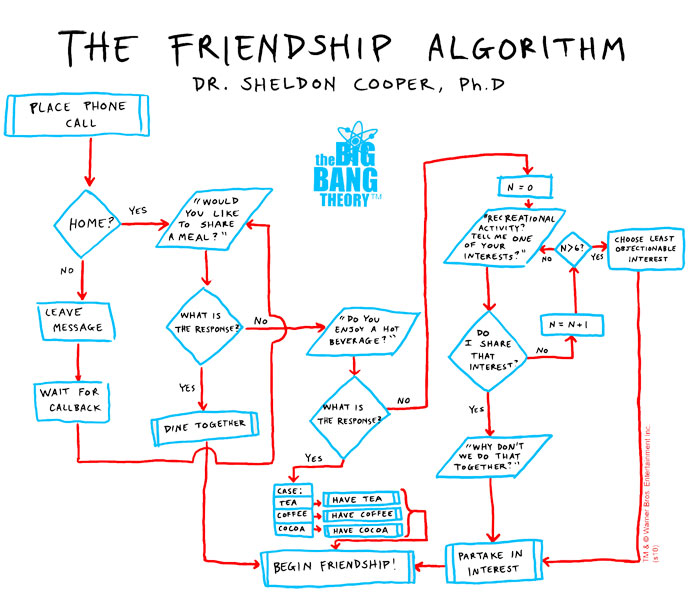
\includegraphics[scale=.27]{../img/friendship.jpg}}
\end{frame}

\section{Relational operators}
\subsection{}
\begin{frame}{The truth about expressions}
	Expressions can also be evaluated to truth values.\\
	If a value or a variable equals 0, its corresponding truth value is \textit{false}. Otherwise it's \textit{true}.\\
	The representations of \textit{false} and \textit{true} are 0 and 1.\\
	An expression containing relational operators gets evaluated to such a truth value.\\
	\ \\Relational operators:
	\begin{itemize}
		\item $<$, $>$, $<$=, $>$=
		\item == for "equal to"
		\item != for "not equal to"
	\end{itemize}
\end{frame}
\begin{frame}[fragile]{Do not get confused}
	Imagine the following
	\begin{lstlisting}[numbers=none]
(5 < 7) =@\,@= 1;	/* evaluated to 1 */
\end{lstlisting}
\ \\\ \\Why?
\begin{itemize}
	\item<2-> (5 $<$ 7) is \textbf{true} $\rightarrow$ \textbf{1}
	\item<3-> 1 == 1 is \textbf{true} $\rightarrow$ \textbf{1}
\end{itemize}
\end{frame}
\begin{frame}[fragile]{A sign meant...}
	Assignments are expressions that get evaluated and have a truth value, too.
	Consider:
		\begin{lstlisting}[numbers=none]
c = 0;				/* 0 -> false */
c = 2 * 5;			/* 2 * 5 = 10,	 c = 10, true */
c = (0 < 1);		/* 0 < 1 = true, c = 1,	 true */

a = (b =@\,@= (c = d));	/* Wat? */
\end{lstlisting}\ \\
	\pause
	\ \\\textit{c++} expressions are evaluated before the increment while \textit{++c} increments first (the same applies on \textit{c$--$} and \textit{$--$c}):
	\begin{lstlisting}[numbers=none]
int c = 42;
int a = c++;	/* evaluates to c,	   a is 42, c is 43 */
int b = ++c;	/* evaluates to c + 1, b is 44, c is 44 */
\end{lstlisting}
\end{frame}
\section{Logical operators}
\subsection{}
\begin{frame}{Boolean arithmetic}
	Truth values can be connected by boolean operators resulting in a new truth value.
	\begin{itemize}
		\item \&\& for AND (results in \textbf{1} if both operands are true, else \textbf{0})
		\item $||$ for OR (results in \textbf{1} if at least one operator is true, else \textbf{0})
		\item ! for NOT (results in \textbf{1} if the operand is false, else \textbf{0})
	\end{itemize}
	\ \\\ \\Precedence order:\\
	\centering
	! \ $>$ \ \&\& \ $>$ \ $||$ 
\end{frame}
\begin{frame}[fragile]{Seems logical}
	\begin{itemize}
		\item How do you get NAND, NOR and XOR?
	\end{itemize}
	\begin{uncoverenv}<2->
		\begin{lstlisting}[numbers=none]
int a, b;
...
!(a && b);	/* NAND */
!(a || b);	/* NOR */
a != b;		/* XOR */
(a == a) != (b == b);	/* safe XOR */
\end{lstlisting}
	\end{uncoverenv}
\end{frame}

\section{Conditions}
\subsection{}
\begin{frame}[fragile]{if...else}
	To make decisions during run time, you can use the truth value of an expression:
	\begin{lstlisting}[numbers=none,basicstyle=\itshape\footnotesize]
if (condition)
	statement1;
else
	statement2;
\end{lstlisting}
	Now \textbf{statement1} is only executed if the truth value of \textbf{condition} is \textit{true}. Otherwise \textbf{statement2} is executed. The \textit{else} part is optional.\\\ \\
	For multiple statements in the \textit{if} or \textit{else body}, use braces:
	\begin{lstlisting}[numbers=none,basicstyle=\itshape\footnotesize]
if (condition) {
	statement1;
	statement2;
}
\end{lstlisting}
\end{frame}
\begin{frame}[fragile]{else if}
	To differentiate between more than two cases, you can use the if condition as a statement in the else body:\\\ \\
	\begin{columns}[c]
		\column{0.5\textwidth}
		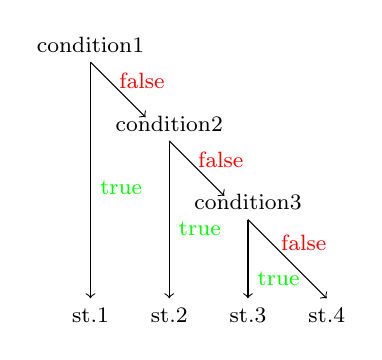
\begin{tikzpicture}[font=\footnotesize]
			\node at (0,0)[above]{condition1};
			\draw[->] (0,0) -- (0,-3) node[green, above=4em, right]{true};
			\node at (0,-3)[below]{st.1};
			\draw[->] (0,0) -- (.7,-.7) node[red, above=1.3em, right=-1.3em]{false};
			
			\node at (1,-1)[above]{condition2};
			\draw[->] (1,-1) -- (1,-3) node[green, above=2.5em, right]{true};
			\node at (1,-3)[below]{st.2};
			\draw[->] (1,-1) -- (1.7,-1.7) node[red, above=1.3em, right=-1.3em]{false};
			
			\node at (2,-2)[above]{condition3};
			\draw[->] (2,-2) -- (2,-3) node[green, above=.7em, right]{true};
			\node at (2,-3)[below]{st.3};
			\draw[->] (2,-2) -- (3,-3) node[red, above=2em, right=-2em]{false};
			
			\node at (3,-3)[below]{st.4};
		\end{tikzpicture}
		\column{0.5\textwidth}
			\begin{lstlisting}[numbers=none,basicstyle=\itshape\footnotesize]
if (condition1)
	statement1;
else if (condition2)
	statement2;
else if (condition3)
	statement3;
else
	statement4;
\end{lstlisting}
	\end{columns}
\end{frame}
\begin{frame}[fragile]{switch}
	If you have to check one variable for many constant values, \textit{switch case} is your friend:
	\begin{lstlisting}[numbers=none,basicstyle=\itshape\footnotesize]
switch (variable) {
	case option1: statement1; break;
	case option2: statement2; break;
	case option3: statement3; break;
	default: statement4; break;
}
\end{lstlisting}
	\begin{itemize}
	\item \textit{case option} defines a jump label
	\item More than one statement after it possible without braces
	\item All statements until the next \textit{break;} will be executed
\end{itemize}	 
\end{frame}
\begin{frame}[fragile]{A few words on style}

	\begin{itemize}
		\item Typing \textbf{if (cond)} instead of \textbf{if(cond)} helps people to differentiate between control structures and function calls faster
		\item When starting a new block, you should type ) \{ rather than )\{
		\item Do not start a new block for a single statement
		\item Do not put statements and conditions on the same line
	\end{itemize}
	\begin{lstlisting}[numbers=none]
if(cond){ statement; }	/* bad style */

if (cond) {				/* looks better, still bad style */
	statement;
}

if (cond)
	statement;			/* looks way clearer */
\end{lstlisting}
\end{frame}
\begin{frame}[fragile]{More words on style}
	\begin{itemize}
		\item if you use a block anywhere in an \textbf{if ... else} structure, put all blocks of this structure in braces
	\end{itemize}
	\begin{lstlisting}[numbers=none]
if (§cond§)		/* bad style, inconsistent */
	§statement§;
else {
	§statement§;
	§statement§;
}

if (§cond§) {		/* way better style */
	§statement§;
} else {
	§statement§;
	§statement§;
}
\end{lstlisting}
\end{frame}

% nothing to do from here on
\end{document}
